\epi{I have this phobia about having my body penetrated surgically. You
know what I mean?}{\textit{eXistenZ}\\\textsc{TED PIKUL}}
\noindent{}
\gomarginpar{The following text is from \cite{go_interfaces}. Written by Ian 
Lance Taylor --- one of the authors of Go.}
In Go, the word \first{\emph{interface}}{interface} is overloaded to mean several different
things. Every type has an interface, which is the \emph{set of methods
defined} for \index{interface!set of methods}
that type. This bit of code defines a struct type \type{S} with one field, and
defines two methods for \type{S}.
\begin{lstlisting}[caption=Defining a struct and methods on it,label=src:interface object]
type S struct { i int }
func (p *S) Get() int { return p.i }
func (p *S) Put(v int) { p.i = v }
\end{lstlisting}
You can also define an \first{interface type}{interface!type}, which is simply a set of methods.
This defines an interface \type{I} with two methods:
\begin{lstlisting}
type I interface {
  Get() int
  Put(int)
}
\end{lstlisting}
\begin{lbar}
An interface type is a set of methods.
\end{lbar}

\type{S} is a valid \emph{implementation} for \type{I}, because it defines the two 
methods which \type{I} requires. Note that this is true even though there is 
no explicit declaration that \type{S} implements \type{I}. A Go program can use 
this fact via yet another meaning of interface, which is an
\first{interface!value}{interface!value}:

\begin{lstlisting}
func f(p I) { fmt.Println(p.Get()); p.Put(1) }
\end{lstlisting}
Here the variable \var{p} holds a value of interface type. Because
\type{S}
implements \type{I}, we can call \func{f} passing in a pointer to a value of type
\type{S}:

\begin{lstlisting}
var s S; f(&s)
\end{lstlisting}
The reason we need to take the address of \type{s}, rather than a value of type
\type{S}, is because we defined the methods on \type{s} to operate on
pointers, see the code above in listing \ref{src:interface object}.
This
is not a requirement --- we could have defined the methods to take
values --- but then the \func{Put} method would not work as expected.

The fact that you do not need to declare whether or not a type implements an
interface means that Go implements a form of 
\first{duck typing}{duck typing}\cite{duck_typing}. 
This is not
pure duck typing, because when possible the Go compiler will statically
check whether the type implements the interface. However, Go does have a
purely dynamic aspect, in that you can convert from one interface type
to another. In the general case, that conversion is checked at runtime.
If the conversion is invalid --- if the type of the value stored in the
existing interface value does not satisfy the interface to which it is
being converted --- the program will fail with a runtime error.

Interfaces in Go are similar to ideas in several other programming languages:
pure abstract virtual base classes in C++, typeclasses in Haskell or duck typing
in Python. However there is no other language which combines
interface values, static type checking, dynamic runtime conversion, and no
requirement for explicitly declaring that a type satisfies an interface. The
result in Go is powerful, flexible, efficient, and easy to write.

\subsection{Empty interface}
For example, since every type satisfies the empty interface:
\type{interface \{\}}. We can create a generic function which 
has an empty interface as its argument:
\begin{lstlisting}[caption=A function with a empty interface argument,label=src:interface empty]
func g(any interface{}) int { 
    return any.(I).Get() 
}
\end{lstlisting}
The \lstinline{return any.(I).Get()} is the tricky bit in this function.
The value \var{any} has type \type{interface{}}, meaning no guarantee
of any methods at all: it could contain any type. The \lstinline{.(I)}
is a \first{type switch}{type switch} which converts \var{any} to an interface of
type \type{I}. If we have that type we can invoke the \func{Get()}
function.
So if we create a new variable of the type \type{*S}, we can just
call \func{g()}, because \type{*S} also implements the empty interface.
\begin{lstlisting}
s = new(S)
fmt.Println(g(s));
\end{lstlisting}
The call to \func{g} will work fine and will print 0. If we however
invoke \func{g()} with a value that does not implement \type{I} we have
a problem:
\begin{lstlisting}[caption=Failing to implement an interface,label=src:interface fail]
i := 5		// make i a "lousy" int
fmt.Println(g(i))
\end{lstlisting}
This compiles OK, but when we run this we get slammed with:

\noindent\error{panic: interface conversion: int is not main.I: missing
method Get}

\noindent{}Which is completely true, the built-in type \type{int} does not
have a \func{Get()} function.

\subsection{Methods}
Methods are functions that have an receiver (see chapter
\ref{chap:functions}).
You can define methods on any type (except the built-ins like
\type{int}) can have methods. 
You can make an integer type with its own methods. For example:
\begin{lstlisting}
type Foo int

func (self Foo) Emit() {
  fmt.Printf("%v", self)
}

type Emitter interface {
  Emit()
}
\end{lstlisting}

Doing this on built-in (are types defined in other package) types yields:
% Empty line here is critical, otherwise no new paragraph is created

\begin{minipage}{.5\textwidth}
\begin{lstlisting}[linewidth=.7\textwidth,caption=Failure extending built-in types]
func (i int) Emit() {
  fmt.Printf("%d", i)
}
\end{lstlisting}
\noindent\error{cannot define new methods\\ on non-local type int}
\end{minipage}
\begin{minipage}{.5\textwidth}
\begin{lstlisting}[caption=Failure extending non-local types]
func (a *net.AddrError) Emit() {
  fmt.Printf("%v", a)
}
\end{lstlisting}
\noindent\error{cannot define new methods\\ on non-local type net.AddrError}
\end{minipage}

\paragraph{}  %% needed otherwise the minipage flows over
Another thing about the receiver; it can not be a defined for interface
types, doing so results in a \error{invalid receiver type ...} compiler
error. The authoritative word from the language spec \cite{go_spec}:
\begin{quote}
The receiver type must be of the form \type{T} or \type{*T} where
\type{T} is a type name. \type{T} is called the receiver base type or just base 
type. The base type must
not be a pointer or interface type and must be declared in the same
package as the method.
\end{quote}

\section{Interface names}
By convention, one-method interfaces are named by the method name plus
the \emph{-er} suffix: Read\emph{er}, Writ\emph{er}, Formatt\emph{er} etc.

There are a number of such names and it's productive to honor them and
the function names they capture. \func{Read}, \func{Write},
\func{Close}, \func{Flush}, \func{String} and
so on have canonical signatures and meanings. To avoid confusion, don't
give your method one of those names unless it has the same signature and
meaning. Conversely, if your type implements a method with the same
meaning as a method on a well-known type, give it the same name and
signature; call your string-converter method \func{String} not
\func{ToString}.
\gomarginpar{Text copied from \cite{effective_go}.}

\section{Introspection}
\label{sec:introspection}
In a program, you can discover the dynamic type of an interface variable
by using a \key{switch}.
Such a type switch\gomarginindex{type switch}{type switch} uses
the syntax of a type assertion with the keyword type inside the
parentheses. If the switch declares a variable in the expression, the
variable will have the corresponding type in each clause.
\begin{lstlisting}[caption=Dynamically find out the type]
package main
type PersonAge struct { |\longremark{First we define two structures as a new type, %
\texttt{PersonAge};}|
	name string
	age  int
}

type PersonShoe struct { |\longremark{And \texttt{PersonShoe};}|
	name     string
	shoesize int
}

func main() {
	p1 := new(PersonAge)
	p2 := new(PersonShoe)
	WhichOne(p1)
	WhichOne(p2)
}

func WhichOne(x interface{}) { |\longremark{This function must accept \emph{both} %
types as valid input, so we use the empty Interface, which every type implements;}|
	switch t := x.(type) { |\longremark{The type switch: \texttt{(type)};}|
	case *PersonAge:	|\longremark{When allocated with \func{new} it's a %
pointer. So we check for \type{*PersonAge}. If \func{WhichOne()} was %
called with a non pointer value, we should check for \type{PersonAge}.}|
		println("Age person")
	case *PersonShoe:
		println("Shoe person")
	}
}
\end{lstlisting}
\showremarks

The following is another example of performing a type switch, but this
time checking for more (built-in) types:
\begin{lstlisting}[caption=A more generic type switch]
switch t := interfaceValue.(type) { |\coderemark{The type switch}|
case bool:
    fmt.Printf("boolean %t\n", t)
case int:
    fmt.Printf("integer %d\n", t)
case *bool:
    fmt.Printf("pointer to boolean %t\n", *t)
case *int:
    fmt.Printf("pointer to integer %d\n", *t)
default:
    fmt.Printf("unexpected type %T", t)  // \%T prints type
}
\end{lstlisting}

\subsection{Introspection and reflection}
\label{subsec:introspection and reflection}
In the following example we want to look at the "tag" (here named
"namestr") defined in the
type definition of \type{Person}. To do this we need the
\package{reflect}\index{package!reflect} package (there is no other way in Go). Keep in mind
that looking at a tag means going back the \emph{type} definition. So
we use the \package{reflect}package to figure out the type of the variable
and \emph{then} access the tag.

\begin{lstlisting}[caption=Introspection using reflection,label=src:introspection]
|\begin{tikzpicture}[overlay]
\draw [->,thick] (2.8,-6.00) node [left] %
{\longremark{We are dealing with a \type{PtrValue} and according %
to the documentation\footnote{\texttt{godoc reflect}}:%
\begin{quote} %
\texttt{\func{func} (v *PtrValue) Elem() Value}\\%
Elem returns the value that v points to. %
If v is a nil pointer, Elem returns a nil Value. %
\end{quote} %
we can use \func{Elem()} to get the type the pointer points to. %
In this case \type{*reflect.StructValue};}} %
to (2.8,-5.20);
%
\draw [->,thick] (3.8,-6.00) node [left] %
{\longremark{\func{Type()} returns \type{reflect.Type};}} %
to (3.8,-5.20);
\draw [->,thick] (5.4,-6.00) node [left] %
{\longremark{%
Again according to the documentation, we have:\\%
\begin{quote} %
\ldots which returns an object with interface %
type \type{Type}.  That contains a pointer to a struct of type %
\type{*StructType}, %
\type{*IntType}, etc. representing the details of the underlying type. %
A type switch or type assertion can reveal which. %
\end{quote} %
So we can access your specific type as a member of this struct. Which %
we do with \type{(*reflect.StructType)};}} %
to (5.4,-5.20);
%
\draw [->,thick] (6.8,-6.00) node [left] %
{\longremark{%
A \type{StructType} has a number of methods, one of which is %
\func{Field($n$)} which returns the $n^{th}$ field of a structure. %
The type of this return is a \type{StructField}; %
}} %
to (6.8,-5.20);
%
\draw [->,thick] (8.4,-6.00) node [left] %
{\longremark{We finally have the type we are after. Now we can use the %
methods defined for \type{*StructType}, like \func{Field(n)}, which %
returns the n$^{th}$ field of our struct as a \type{StructField};}} %
to (8.4,-5.20);
%
\draw [->,thick] (9.4,-6.00) node [left] %
{\longremark{The struct \type{StructField} has a \var{Tag} member which %
returns the tag-name as a string. So on the $0^{th}$ field we can %
unleash \func{.Tag} to access this name: \texttt{Field(0).Tag}. This %
\emph{finally} gives us \texttt{namestr}.}}%
to (9.4,-5.20);
\end{tikzpicture}|
type Person {
    name string "namestr"
    age  int
}

p1 := new(Person)   |\coderemark{\func{new} returns a pointer to Person}|
ShowTag(p1)	    |\coderemark{\func{ShowTag()} is now called with this pointer}|

func ShowTag(i interface{}) {
    switch t := reflect.NewValue(i).(type) { |\coderemark{Type assertion}|
    case *reflect.PtrValue:		     |\coderemark{\var{p1} is a pointer}|
	tag := t.Elem().Type().(||*reflect.StructType).Field(0).Tag
||
\end{lstlisting}

\showremarks

%% look at layout
To make the difference between looking a types and values more clear,
that a look at the following code:
\begin{lstlisting}[caption=Reflection and the type and value]
func show(i interface{}) {
    switch t := i.(type) {
      case *Person:
        r := reflect.NewValue(i) |\coderemark{Enter the world of reflection}|
	tag := |\longremark{Here we want to get the "tag", which means %
going for the type. Thus we need\newline\lstinline{Elem().Type().(*reflect.StructType)} to get to it;}|
	  r.(*reflect.PtrValue).Elem().Type().(*reflect.StructType).Field(0).tag
	nam := |\longremark{Now we want to get access to the %
\emph{value} of one of the members and we %
employ\newline\lstinline{Elem().(*reflect.StructValue)} to get to it. %
Now we have arrived at the structure. Then we go the the first field %
\lstinline{Field(0)}, tell \package{reflect} is a %
\var{*reflect.StringValue} and invoke the \lstinline{Get()} method on %
it. %
\begin{figure}[H] %
\hskip3\baselineskip\parbox{0.7\textwidth}{\caption[Pealing away the layers using reflection]{Pealing away the %
layers using reflection. %
Going from a \type{*Person} via \mbox{\type{*reflect.PtrValue}} using the %
methods described in \prog{godoc reflect} to get the %
actual \type{string} contained deep within.}} %
\label{fig:reflection} %
\begin{center} %
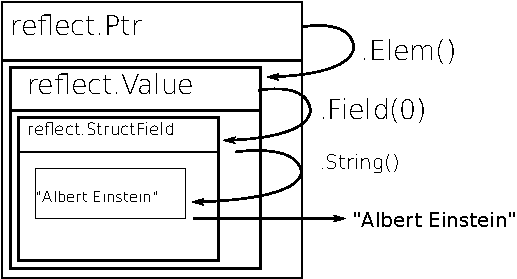
\includegraphics[scale=0.75]{fig/reflection.pdf} %
\end{center}\end{figure} %
Reflection works by pealing off layers once you have got your hands %
on a \type{Value} in the reflection world.}|
	  r.(*reflect.PtrValue).Elem().(*reflect.StructValue).Field(0)\newline.(*reflect.StringValue).Get()
    }
}
\end{lstlisting}
\showremarks

Setting a value works similarly as getting a value, but only works on
\emph{exported} members. Again some code:

\begin{minipage}{.5\textwidth}
\begin{lstlisting}[caption=Reflect with private member]
type Person struct {
 name string "namestr"
 age  int
}

func Set(i interface{}) {
 switch t := i.(type) {
 case *Person:
  r := reflect.NewValue(i)
  r.(*reflect.PtrValue).Elem().
    (*reflect.StructValue).
    FieldByName("name").
    (*reflect.StringValue).
    Set("Albert Einstein")
  }
}
\end{lstlisting}
\end{minipage}
\hspace{2em}
\begin{minipage}{.5\textwidth}
\begin{lstlisting}[caption=Reflect with public member]
type Person struct {
 Name string "namestr" |\coderemark{}|
 age  int
}

func Set(i interface{}) {
 switch t := i.(type) {
 case *Person:
  r := reflect.NewValue(i)
  r.(*reflect.PtrValue).Elem().
   (*reflect.StructValue).
   FieldByName("Name"). |\coderemark{}|
   (*reflect.StringValue).
   Set("Albert Einstein")
  }
}
\end{lstlisting}
\end{minipage}
The code on the left compiles and runs, but when you run it, you are greeted with a
stack trace and a \emph{runtime} error:

\noindent\error{panic: cannot set value obtained via unexported struct
field}

\noindent{}The code on the right works OK and sets the member \var{Name}
to "Albert Einstein". Of course this only works when you call \func{Set()}
with a pointer argument.

\section{A sorting example}
Recall the Bubblesort exercise (Q\ref{ex:bubble}), where we sorted an
array of integers:
\begin{lstlisting}
func bubblesort(n []int) {
    for i := 0; i < len(n); i++ {
	for j := i; j < len(n); j++ {
	    if n[j] < n[i] {
		    n[i], n[j] = n[j], n[i]
	    }
	}
    }
}
\end{lstlisting}
A version that sorts strings is identical except for the signature of
the function:
\begin{lstlisting}
func bubblesortString(n []string) { /* ... */ }
\end{lstlisting}
Now we want to create a new function that will sort both strings and
integers, something along the lines:
\begin{lstlisting}
func sort(i []interface{}) {
    switch i.(type) {
	case string:
	    // convert to string
	case int:
	    // convert to int
    }
    // sort
    // return sorted array
}
\end{lstlisting}
But when we call this function with \lstinline|sort([]int{1, 4, 5})|, it
fails with
\error{cannot use i (type []int) as type []interface { } in function argument}

This is because Go will implicitly convert an \type{int} or
\type{string} (or whatever) to an interface, as this is very easy to
do. But converting a slice is much more costly. Also when
converting a slice the content is copied to another slice and thus
that new slice refers to a different array. To keep a 
\gomarginpar{the full mailing list discussion on this subject
can be found at \cite{go_nuts_interfaces}.}
long story short: Go does not (implicitly) convert slices for you.

So what is the Go way of creating such a "generic" function? 
Instead of doing the type inference our selves, we handover 
that task to Go by using interfaces.
The following steps are required:
\begin{enumerate}
\item Define an interface type (called \type{S} here) with a number of 
methods needed for sorting.
We will at least need a function to get the length of the array,
a function to compare two values and a swap function;
\begin{lstlisting}
type S interface {
    Len() int           // len() as a method
    Less(i, j int) bool // <     as a method
    Swap(i, j int)      // p[i], p[j] = p[j], p[i] as a method
}
\end{lstlisting}
\item Define new types for the arrays we want to sort. We need this
because we can not declare methods on built-in types;
\begin{lstlisting}
type Xi []int
type Xs []string
\end{lstlisting}
\item Implement the methods of the \type{S} interface.
For integers:
\begin{lstlisting}
func (p Xi) Len() int               { return len(p) }
func (p Xi) Less(i int, j int) bool { return p[i] < p[j] }
func (p Xi) Swap(i int, j int)      { p[i], p[j] = p[j], p[i] }
\end{lstlisting}
And for strings;
\begin{lstlisting}
func (p Xs) Len() int               { return len(p) }
func (p Xs) Less(i int, j int) bool { return p[i] < p[j] }
func (p Xs) Swap(i int, j int)      { p[i], p[j] = p[j], p[i] }
\end{lstlisting}
\item Write a generic Sort function that works on the \type{S} interface.
\begin{lstlisting}
func Sort(x S) {
    for i := 0; i < x.Len(); i++ {
	for j := i; j < x.Len(); j++ {
	    if x.Less(i, j) {
		x.Swap(i, j)
	    }
	}
    }
}
\end{lstlisting}
\end{enumerate}
We can now use you generic \func{Sort} function as follows:
\begin{lstlisting}
ints := Xi{44, 67, 3, 17, 89, 10, 73, 9, 14, 8}
strings := Xs{"noot", "aap", "mies", "miek", "Go"}

Sort(ints)
fmt.Printf("%v\n", ints)
Sort(strings)
fmt.Printf("%v\n", strings)
\end{lstlisting}

\section{Exercises}
\begin{Exercise}[title={接口和编译},difficulty=1]
\Question
在第 \pageref{src:interface fail} 页的代码 \ref{src:interface fail} 
编译正常——就像文中开始描述的那样。但是当运行的时候,会得到运行时错误,
因此有些东西\emph{有}错误。为什么代码编译没有问题呢?
\end{Exercise}

\begin{Answer}
\Question
代码能够编译是因为整数类型实现了空接口,这是在编译时检查的。

修复这个正确的途径是测试这个空接口可以被转换,如果可以,调用对应的方法。
\ref{src:interface empty} 列出的 Go 代码中定义了函数 \func{g}——这里重复一下:
\begin{lstlisting}
func g(any interface{}) int { return any.(I).Get() }
\end{lstlisting}

\noindent{}应当修改为:
\begin{lstlisting}
func g(any interface{}) int {
    if v, ok := any.(I); ok {	// 检查是否可以转换
	return v.Get()		// 如果可以,调用 Get()
    }
    return -1			// 随便返回个什么
}
\end{lstlisting}
如果现在调用 \func{g()},就不会有运行时错误了。在 Go 中这种用法被称作``comma ok''。
\end{Answer}


\begin{Exercise}[title={接口和最大最小},difficulty=1]
\Question
构造一个通用的最大最小,使得可以同时工作于整数和字符串,就像第 \titleref{sec:a sorting example} 节中那样。
\end{Exercise}

\begin{Answer}
\Question
\end{Answer}


\cleardoublepage
\section{Answers}
\shipoutAnswer
